% \fakesubsection{V-Model}
\flushleft
\textbf{V-Model}\\
\justifying

\parx
The V-model process is a software development process which is an extension of
the traditional waterfall model. The model shows the relationships between each
of the different phases in the life cycle of the development process, each with
an associated testing phase. After the linear top to bottom phases are complete,
the process proceeds to bottom to top phases for testing and to complete the
model cycle. The V-model is a well-structured method in which each phase is
implemented following the documentation provided previously. The primary focus
and purpose of this model is to improve the efficiency of development and to
ensure the effectiveness by following the relationship of each phase with its
associated testing phase (\cite{rook_1986}).

\parx
The traditional V-model is composed of the following phases:

\begin{figure}[H]
	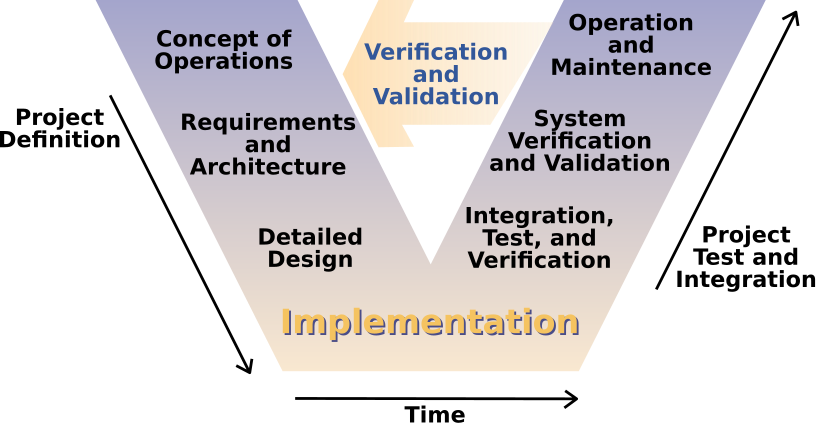
\includegraphics[width=\linewidth]{figures/v_model.png}
	\caption{V-Model}
	\label{fig:v_model}
\end{figure}

\parx
\textbf{Requirements.}
\justifying
Involves the gathering of data, analysis of the gathered data, and preparation
of the system requirements in defining the scope and features of the project.
This stage also involves the documentation of the requirements.

\parx
\textbf{System Design.}
\justifying
The documents created in the previous stage will be used to generate more
specific and technical documents and designs about the software to be developed
for this stage. The documents outline the components, modules, and high-level
guidelines for business logic.

\parx
\textbf{Architecture Design.}
\justifying
The technical designs from the System Design stage will be used to generate
specifications with lower level of technical details about the software and its
modules. The technology stack is also selected in this stage. During this stage,
the tests are also prepared for future use.

\parx
\textbf{Module Design.}
\justifying
In this stage, low-level designs are developed from the high-level designs
generated from previous stages. This will include specifications regarding each
individual module, component, interface, and so on. Unit tests are also prepared
in this stage.

\parx
\textbf{Implementation and Coding.}
\justifying
This stage the implementation through programming starts. It starts with coding
the each module individually with unit tests along applied following the designs
made in the initial stages of the development life cycle. Integration of the
modules to the system is done afterward and is run through system tests.

\parx
\textbf{Testings.}
\justifying
Tests are further applied to the system such as unit testing, integration
testing, system testing, and acceptance testing. Passing all these tests will be
considered as the verification and validation of the project.
